\documentclass[12pt]{article}
\usepackage{geometry}                % See geometry.pdf to learn the layout options. There are lots.
\geometry{letterpaper}                   % ... or a4paper or a5paper or ... 
%\geometry{landscape}                % Activate for for rotated page geometry
\usepackage[parfill]{parskip}    % Activate to begin paragraphs with an empty line rather than an indent
\usepackage{daves,fancyhdr,natbib,graphicx,dcolumn,amsmath,lastpage,url}
\usepackage{amsmath,amssymb,epstopdf,longtable}
\usepackage{paralist} 
\DeclareGraphicsRule{.tif}{png}{.png}{`convert #1 `dirname #1`/`basename #1 .tif`.png}
\pagestyle{fancy}
\lhead{CE 3372 -- Water Systems Design}
\rhead{FALL 2020}
%\rhead{FALL 2016}
%\rhead{SPRING 2016}
%\rhead{FALL 2011}
%\rhead{SPRING 2012}
%\rhead{FALL 2012}
%\rhead{FALL 2015}
%\rhead{FALL 2010}
%\lfoot{EXERCISE 1 -- REVISION 1}
%\lfoot{EXERCISE 1 -- REVISION 2}
%\lfoot{EXERCISE 1 -- REVISION 3}
%\lfoot{EXERCISE 1 -- DUE 26 JAN 2012}
%\lfoot{EXERCISE 1 -- DUE 4 SEP 2012}
\lfoot{EXERCISE 4}
\cfoot{}
\rfoot{Page \thepage\ of \pageref{LastPage}}
\renewcommand\headrulewidth{0pt}
\newcommand\tab[1][1cm]{\hspace*{#1}}


\begin{document}
\begin{center}
{\textbf{{ CE 3372 -- Water Systems Design} \\ {Exercise Set 4}}}
\end{center}
\begingroup
\begin{tabular}{p{1in} p{5in}}
Purpose: & Closed conduit hydraulics and use of energy equation for water distribution systems analysis \\
~& Application of head loss models in water distribution system analysis \\

\end{tabular}
\endgroup
\section*{\small{Exercises}}
\begin{enumerate}
%%%%%%%%%%%%%%%% TEXAS ADMINISTRATIVE CODE %%%%%%%%%%%%%%%%%%%%%%%%%%%%%%%%%%%%%%%%%%%%%%%%%%%%%%

\item Equation \ref{eqn:hazen-williams} is the  Hazen-Williams discharge formula in US Customary Units. 
\begin{equation}
Q = 1.318 C_h A R^{0.63} S^{0.54}
\label{eqn:hazen-williams}
\end{equation}
where;\\
\tab $Q$ is the discharge in $ft^3/sec$;\\
\tab $A$ is the cross section area of pipe in $ft^2$ ($A = \frac{\pi D^2}{4}$; $D$ is the pipe diameter.);\\
\tab $C_h$ is the Hazen-Williams friction coefficient (depends on pipe roughness);\\
\tab $R$ is the hydraulic radius in $ft$; and \\
\tab $S$ is the slope of the energy grade line ($\frac{h_f}{L}$); $L$ is the length of pipe.
\begin{enumerate}[(a)]
%\item Rearrange the equation in terms of head loss ($h_f = \dots$). 
\item Look up the Hazen-Williams loss coefficient ($C_h$) for enamel coated, steel pipe and cite your data source.
\item Estimate the head loss in a 10,000 foot length of 5-foot diameter, enamel coated steel pipe that carries carries 60$^o$F water at a discharge of 295 cubic-feet per second (cfs), using the Hazen-Williams head loss model.
\end{enumerate}
\clearpage
\item Equation \ref{eqn:hazen-williamsSI} is the  Hazen-Williams discharge formula in SI Units. 
\begin{equation}
Q = 0.849 C_h A R^{0.63} S^{0.54}
\label{eqn:hazen-williamsSI}
\end{equation}
where;\\
\tab $Q$ is the discharge in $m^3/sec$;\\
\tab $A$ is the cross section area of pipe in $m^2$ ($A = \frac{\pi D^2}{4}$; $D$ is the pipe diameter.);\\
\tab $C_h$ is the Hazen-Williams friction coefficient (depends on pipe roughness);\\
\tab $R$ is the hydraulic radius in $m$; and \\
\tab $S$ is the slope of the energy grade line ($\frac{h_f}{L}$); $L$ is the length of pipe.
\begin{enumerate}[(a)]
%\item Rearrange the equation in terms of head loss ($h_f = \dots$). 
\item Look up the Hazen-Williams loss coefficient ($C_h$) for Acrylonite Butadiene Styrene (ABS) pipe and cite your data source.
\item Estimate the head loss in a 3,050 meter length of 1.5-meter diameter, ABS pipe that carries carries 20$^o$C water at a discharge of 8.35 cubic-meters per second (cms), using the Hazen-Williams head loss model.
\end{enumerate}
\clearpage
%%%%%%%%%%%%%%%%%%%%%%%%%%%%%%%%%%%%%%%%%%%%%%%%%%%%%%%%%%%%%%%%%%%%%%%%%%%%%%%%%%%%%%%%%%%%%%%%%%%%%
\item 
Equation \ref{eqn:flow-jain} is an explicit formula (based on the Darcy-Weisbach head loss model and the Colebrook-White frictional loss equation)for estimating discharge from head loss and material properties \citep{jain1976}.
\begin{equation}
Q=-2.22D^{5/2} \times \sqrt{gh_f/L}\times[log_{10} (\frac{k_s}{3.7D} + \frac{1.78\nu}{D^{3/2}\sqrt{gh_f/L}} )]
\label{eqn:flow-jain}
\end{equation}

where;\\~\\
\tab $Q$ is the discharge in $L^3/T$;\\
\tab $D$ is the pipe diameter; \\
\tab $h_f$ is the head loss in the pipe; \\
\tab $g$ is the gravitational acceleration constant; \\
\tab $L$ is the length of pipe; \\
\tab $k_s$ is the pipe roughness height; \\
\tab $\nu$ is the viscosity of liquid in the pipe; \\ 


\begin{enumerate}[(a)]
\item Find the viscosity for water at 50$^o$F.  Cite the source of your value. 
\item Find the sand roughness height of ductile iron pipe.  Cite the source of your value. 
\item How deep is a column of water if the pressure at the bottom of the column is 20 psi?
\item Estimate the discharge in the 3 mile long, 24-inch diameter, ductile iron pipeline connecting points A and B depicted in Figure \ref{fig:PipePressureProblem}.  Point A is 30 feet higher in elevation than point B.  The pressure at point B is 20 pounds per square-inch (psi) greater than the pressure at point A.
\end{enumerate}

\begin{figure}[htbp] %  figure placement: here, top, bottom, or page
   \centering
   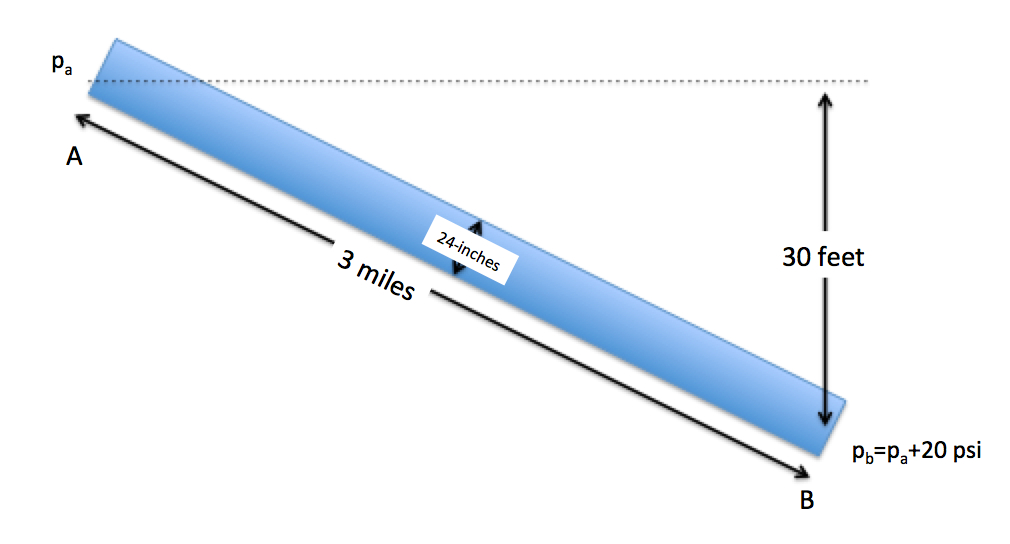
\includegraphics[width=4in]{PipePressureProblem.jpg} 
   \caption{Pipeline Schematic}
   \label{fig:PipePressureProblem}
\end{figure}
\clearpage
%%%%%%%%%%%%%%%%%%%%%%%%%%%%%%%%%%%%%%%%%%%%%%%%%%%%%%%%%%%%%%%%%%%%%%%%%%%%%%%%%%%%%%%%%%%%%%%%%%%%%%%
\item 
Equation \ref{eqn:diameter-jain} is a formula to estimate the required pipe diameter for a particular discharge, head loss, and roughness \citep{jain1976}.
\begin{equation}
D=0.66[k_s^{1.25}\times(\frac{LQ^2}{gh_f})^{4.75}+\nu Q^{9.4}\times(\frac{L}{gh_f})^{5.2}]^{0.04}
\label{eqn:diameter-jain}
\end{equation}

where;\\~\\
\tab $D$ is the pipe diameter; \\
\tab $k_s$ is the pipe roughness height; \\
\tab $L$ is the length of pipe; \\
\tab $g$ is the gravitational acceleration constant; \\
\tab $Q$ is the discharge in $L^3/T$;\\
\tab $h_f$ is the head loss in the pipe; \\
\tab $\nu$ is the viscosity of liquid in the pipe; \\ 

\begin{enumerate}[(a)]
\item Find the viscosity for water at 60$^o$F.  Cite the source of your value.
\item Find the sand roughness height of cast-iron pipe.  Cite the source of your value. 
\item Estimate the diameter of a cast-iron pipe needed to carry 60$^o$F water at a discharge of 10 cubic-feet per second (CFS) between two reservoirs 2 miles apart with an elevation difference between the water surfaces in the two reservoirs of 20 feet as depicted in Figure \ref{fig:PipeLine2Reservoirs}.
\end{enumerate}

\begin{figure}[htbp] %  figure placement: here, top, bottom, or page
   \centering
   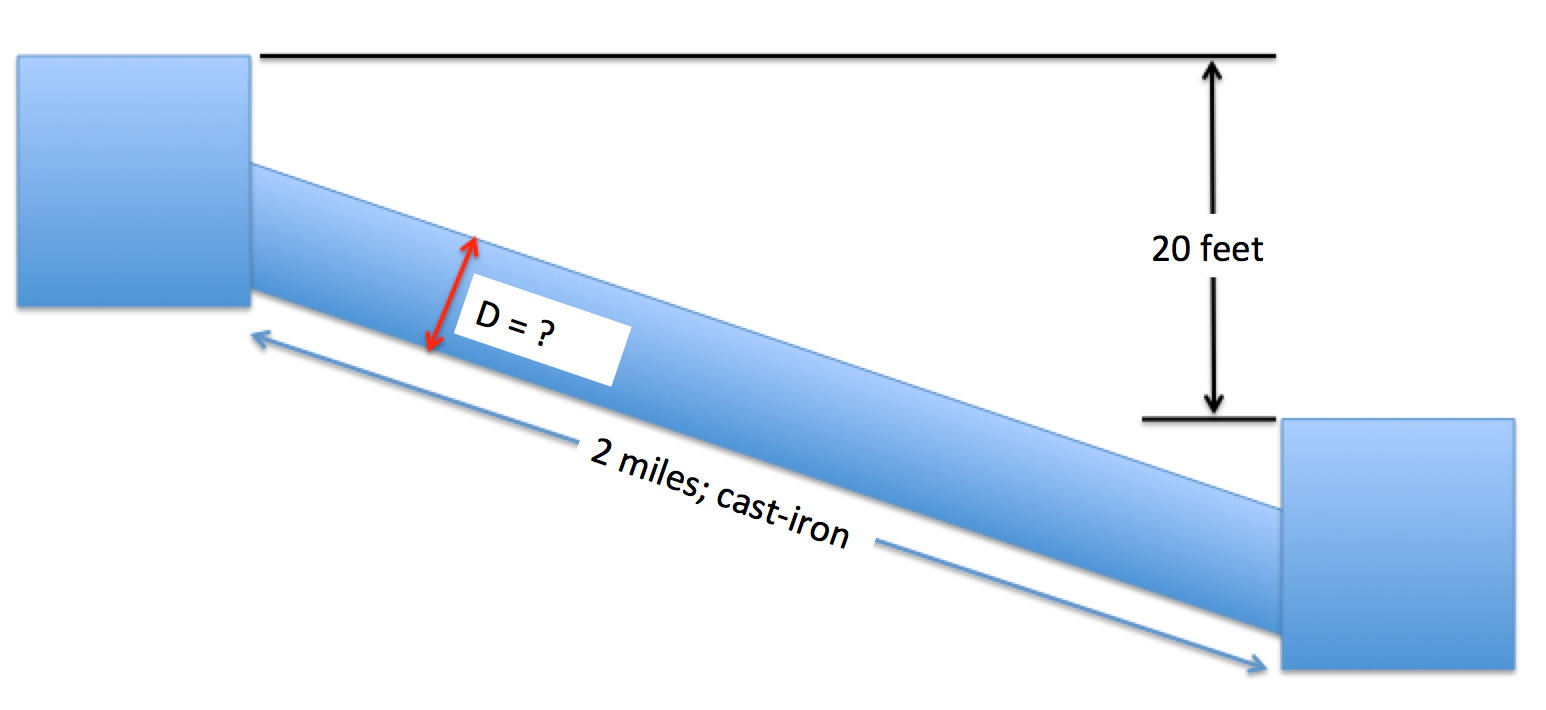
\includegraphics[width=4in]{PipeLine2Reservoirs.jpg} 
   \caption{Pipeline connecting two reservoirs}
   \label{fig:PipeLine2Reservoirs}
\end{figure}
\clearpage
\item A water supply system draws from a river at an elevation of 800-feet and delivers the water to a storage reservoir at elevation 820-feet.  The supply pipeline is a 1000-foot long, 10-inch diameter, cast iron pipe.  A single pump with the pump characteristic curve in Figure \ref{fig:PumpCurve} is used to fill the reservoir.

Determine:
\begin{enumerate}[a)]
\item Sketch the system described in the problem statement.
\item Inlet and outlet minor loss coefficients, cite your source of minor loss coefficients.
\item The roughness ratio for use in the Moody chart, cite your source of roughness height.
\item The energy equation for the system.
\item The system loss for a discharge of 1200, 1600, 2000, 2400, and 2800 gallons-per-minute.  Show the calculation of Reynolds number for the different flow rates.  Show the the friction factors on the attached Moody chart (Figure \ref{fig:moody}).
\item The operating discharge for the system using the supplied pump curve.
\item The electric power supplied to the pump to lift the water at the operating point.\footnote{Assume the efficiency on the pump curve is representative of the wire-to-water efficiency.}
\end{enumerate}

\begin{figure}[h!] %  figure placement: here, top, bottom, or page
\centering
   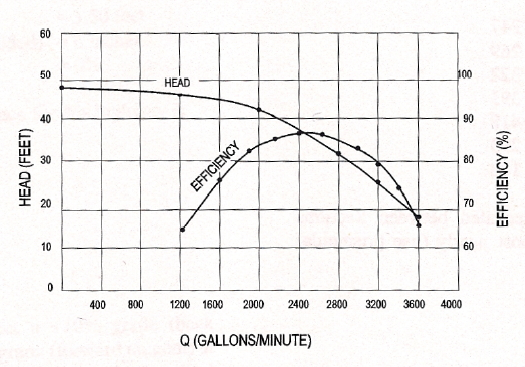
\includegraphics[width=4.5in]{PumpCurve.jpg}
   \caption{Pump characteristic curve}
   \label{fig:PumpCurve} 
\end{figure}

\clearpage
\begin{figure}[h!] %  figure placement: here, top, bottom, or page
\centering
   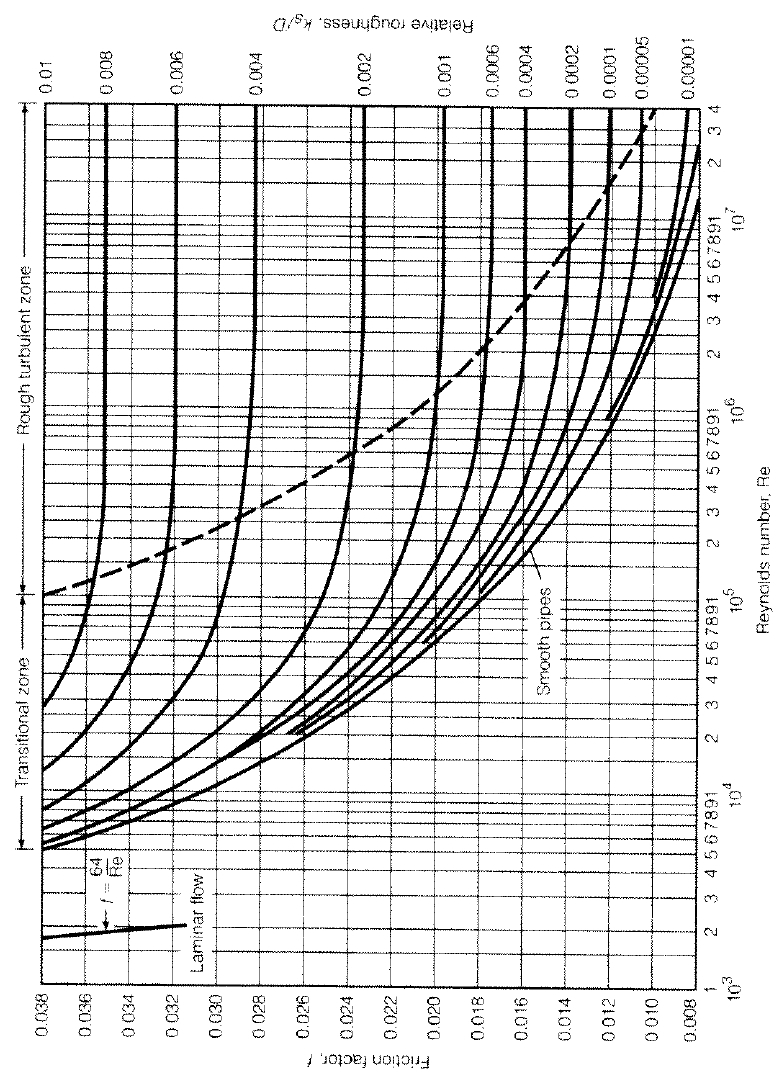
\includegraphics[width=5.5in]{Moody1.jpg}
   \caption{Moody-Stanton Chart}
   \label{fig:moody} 
\end{figure}
\clearpage

%%%%%%%%%%%%%%%%%%%%%%%%%%%%%%%%%%%%%%%%%%%%%%%%%%%%%%%%%%%%%%%%%%%%%%%%%%%%%%%%%%%%%%%%%%%%%%%%

%\item  Water is pumped from a supply reservoir to a ductile iron water-transmission line as shown in Figure \ref{fig:p219}.   The high elevation of the line is at point A, 1 kilometer downstream of the pump station, and the low elevation is at point B, 1 kilometer downstream of point A.  If the discharge in the pipeline is 1 cubic-meter per second (cms), the diameter of the pipe is 750 millimeters (mm) and the pressure at point A is 350 kilopascals (kPa).  Determine
%
%\begin{enumerate}[(a)]
%\item The added head supplied by the pump station.
%\item The water pressure at B.
%\item The mechanical power supplied by the pump.
%\end{enumerate}
%
%\begin{figure}[htbp] %  figure placement: here, top, bottom, or page
%   \centering
%   \includegraphics[width=4in]{p219.pdf} 
%   \caption{Reservoir-Pump-Transmission System Schematic}
%   \label{fig:p219}
%\end{figure}
%\clearpage
%~\\

%%%%%%%%%%%%%%%%%%%%%%%%%%%%%%%%%%%%%%%%%%%%%%%%%%%%%%%%%%%%%%%%%%%%%%%%%%%%%%
\item Figure \ref{fig:water_network_layout} is a layout of a water distribution system for the subdivision.   
The blue line segments are pipes and are labeled (P1, P2, $\dots$).   
The blue circles are nodes and are labeled (N1, N2, $\dots$).
The yellow polygons represent the demand lots assigned to each node.  
For example, node N2 supplies the six (6) individual lots located near the node.
\begin{figure}[ht!] %  figure placement: here, top, bottom, or page
   \centering
   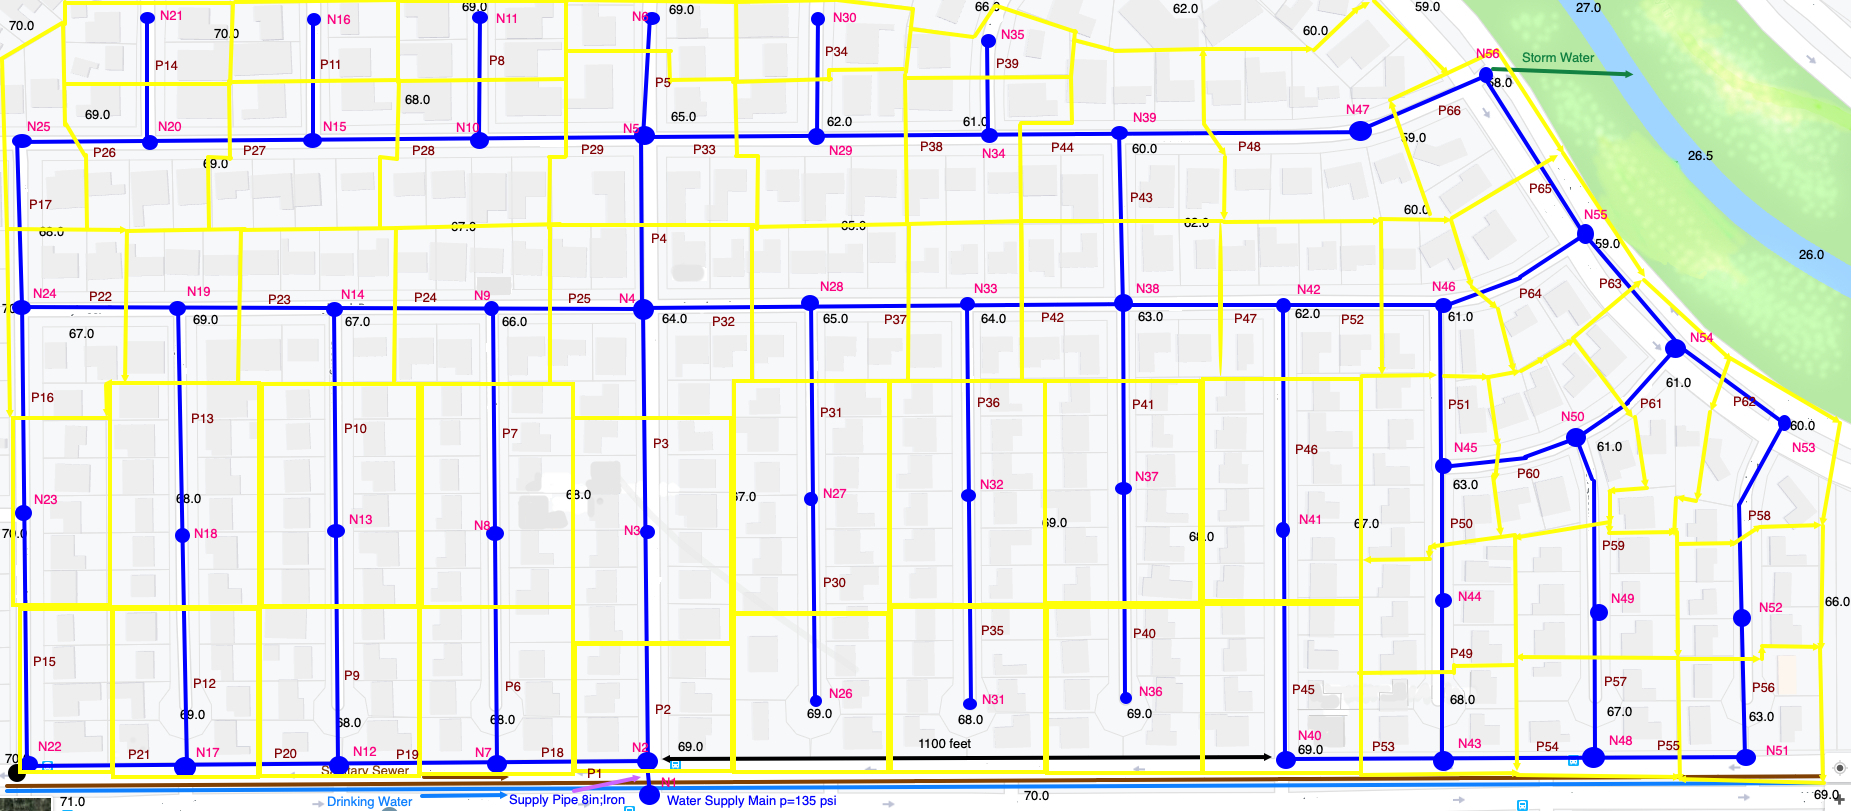
\includegraphics[width=6.5in]{SomewhereClipNodes.jpg} 
   \caption{Water Distribution (Skeleton) System.}
   \label{fig:water_network_layout}
\end{figure}
\begin{enumerate}[a)]
\item Determine the length of each pipe in the sketch.
\item Select an appropriate material for each pipe using San Marcos, Texas water system design guidelines and determine an appropriate Hazen-William's loss coefficient for each pipe.
\end{enumerate}
Use your values to produce a completed version of Table \ref{tab:ByPipes}.
Save the table (in Excel or something similar) -- you will need it later in the design project RP-1.
% Requires the booktabs if the memoir class is not being used
\begin{table}[h!]
   \centering
   \caption{Pipe Properties for Somewhere USA Distribution System}
   \begin{tabular}{p{1in}p{1in}p{1in}p{1in}p{1in}p{1in}} % Column formatting, @{} suppresses leading/trailing space
Pipe ID & L (feet) & D (inches) & Material & $C_H$ & $k_s$ (inches) \\
\hline
\hline
P1 & 44 & 8 & Ductile Iron & 130 & 0.0024 \\
P2 & 440 & 2 &Ductile Iron & 130 & 0.0024 \\
P3 & 385 & 2 &Ductile Iron & 130 & 0.0024  \\
P4 & $\dots$ & 2 &Ductile Iron & 130 & 0.0024  \\
P5 & $\dots$ & 2 &Ductile Iron & 130 & 0.0024  \\
P6 & $\dots$ & 2 &Ductile Iron & 130 & 0.0024  \\
P7 & $\dots$ & 2 &Ductile Iron & 130 & 0.0024  \\
P8 & $\dots$ & 2 &Ductile Iron & 130 & 0.0024  \\
P9 & $\dots$ & 2 &Ductile Iron & 130 & 0.0024  \\
P10 & $\dots$ & 2 &Ductile Iron & 130 & 0.0024  \\
P11 & $\dots$ & 2 &Ductile Iron & 130 & 0.0024  \\
P12 & $\dots$ & 2 &Ductile Iron & 130 & 0.0024  \\
P13 & $\dots$ & 2 &Ductile Iron & 130 & 0.0024  \\
P14 & $\dots$ & 2 &Ductile Iron & 130 & 0.0024 \\
P15 & $\dots$ & 2 &Ductile Iron & 130 & 0.0024  \\
%P16 & ~ & ~ & ~ & ~ & ~ \\
%P17 & ~ & ~ & ~ & ~ & ~ \\
%P18 & ~ & ~ & ~ & ~ & ~ \\
%P19 & ~ & ~ & ~ & ~ & ~ \\
%P20 & ~ & ~ & ~ & ~ & ~ \\
%P21 & ~ & ~ & ~ & ~ & ~ \\
%P22 & ~ & ~ & ~ & ~ & ~ \\
%P23 & ~ & ~ & ~ & ~ & ~ \\
%P24 & ~ & ~ & ~ & ~ & ~ \\
%P25 & ~ & ~ & ~ & ~ & ~ \\
%P26 & ~ & ~ & ~ & ~ & ~ \\
$\dots$ & $\dots$ & $\dots$& $\dots$&$\dots$& $\dots$ \\
$\dots$ & $\dots$ & $\dots$& $\dots$&$\dots$& $\dots$ \\
$\dots$ & $\dots$ & $\dots$& $\dots$&$\dots$& $\dots$ \\
%P27 & ~ & ~ & ~ & ~ & ~ \\
%P28 & ~ & ~ & ~ & ~ & ~ \\
%P29 & ~ & ~ & ~ & ~ & ~ \\
%P30 & ~ & ~ & ~ & ~ & ~ \\
%P31 & ~ & ~ & ~ & ~ & ~ \\
%P32 & ~ & ~ & ~ & ~ & ~ \\
%P33 & ~ & ~ & ~ & ~ & ~ \\
%P34 & ~ & ~ & ~ & ~ & ~ \\
%P35 & ~ & ~ & ~ & ~ & ~ \\
%P36 & ~ & ~ & ~ & ~ & ~ \\
%P37 & ~ & ~ & ~ & ~ & ~ \\
%P38 & ~ & ~ & ~ & ~ & ~ \\
%P39 & ~ & ~ & ~ & ~ & ~ \\
%P40 & ~ & ~ & ~ & ~ & ~ \\
%P41 & ~ & ~ & ~ & ~ & ~ \\
%P42 & ~ & ~ & ~ & ~ & ~ \\
%P43 & ~ & ~ & ~ & ~ & ~ \\
%P44 & ~ & ~ & ~ & ~ & ~ \\
%P45 & ~ & ~ & ~ & ~ & ~ \\
%P46 & ~ & ~ & ~ & ~ & ~ \\
P57 & $\dots$ & 2 &Ductile Iron & 130 & 0.0024  \\
P58 & $\dots$ & 2 &Ductile Iron & 130 & 0.0024  \\
P59 & $\dots$ & 2 &Ductile Iron & 130 & 0.0024  \\
P60 & $\dots$ & 2 &Ductile Iron & 130 & 0.0024  \\
P61 & $\dots$ & 2 &Ductile Iron & 130 & 0.0024  \\
P62 & $\dots$ & 2 &Ductile Iron & 130 & 0.0024  \\
P63 & $\dots$ & 2 &Ductile Iron & 130 & 0.0024  \\
P64 & $\dots$ & 2 &Ductile Iron & 130 & 0.0024  \\
P65 & $\dots$ & 2 &Ductile Iron & 130 & 0.0024  \\
P66 & $\dots$ & 2 &Ductile Iron & 130 & 0.0024  \\
\hline
   \end{tabular}

   \label{tab:ByPipes}
\end{table}

\end{enumerate}
\clearpage
\begin{thebibliography}{}

\bibitem[\protect\citeauthoryear{Swamee and Jain}{Swamee and Jain}{1976}]{jain1976}
Swamee and Jain, A. K., 1976. Explicit equations for pipe-flow problems.  ASCE J. of Hyd. Div., 102(HY5) pp. 657-664 


\end{thebibliography}


\end{document}  